\documentclass[10pt,twocolumn,letterpaper]{article}

\usepackage{cvpr}
\usepackage{times}
\usepackage{epsfig}
\usepackage{graphicx}
\usepackage{amsmath}
\usepackage{amssymb}

% Include other packages here, before hyperref.

% If you comment hyperref and then uncomment it, you should delete
% egpaper.aux before re-running latex.  (Or just hit 'q' on the first latex
% run, let it finish, and you should be clear).
\usepackage[breaklinks=true,bookmarks=false]{hyperref}

\cvprfinalcopy % *** Uncomment this line for the final submission

\def\cvprPaperID{****} % *** Enter the CVPR Paper ID here
\def\httilde{\mbox{\tt\raisebox{-.5ex}{\symbol{126}}}}

% Pages are numbered in submission mode, and unnumbered in camera-ready
%\ifcvprfinal\pagestyle{empty}\fi
\setcounter{page}{1}
\begin{document}

%%%%%%%%% TITLE
\title{Structural Conditioning in Latent Diffusion Models \\for Forensic Scene Reconstruction}

\author{Riccardo Pilan\\
{\tt\small riccardo.pilan@studenti.unipd.it}
}

\maketitle
%\thispagestyle{empty}

%%%%%%%%% ABSTRACT
\begin{abstract}
	
	Text-to-image models have revolutionized the field of generative AI, as they are capable of generating high-fidelity images from simple text prompts. 
    This essay, in particular, analyzes the structure of Latent Diffusion Models (LDMs) for image generation, which are models operating in latent spaces, instead of pixel spaces.
    We will discuss how these models work and consider some of their main strengths, such as their excellent zero-shot generation and semantic understanding, but also critical aspects, such as spatial ambiguity. 
    Then, we will see how ControlNet addresses spatial control issues by introducing explicit spatial conditioning.
    Finally, starting from this approach, we will describe a potential application of the model in the field of forensic science: combining eyewitness testimonies (text prompts) and accurate crime scene data (spatial conditioning) to generate detailed visual reconstructions for investigative hypotheses.
\end{abstract}

%%%%%%%%% BODY TEXT
\section{Introduction}

The rapid advancement of Generative Artificial Intelligence in the last few years has led to remarkable breakthroughs in the field of Computer Vision, and in particular in text-to-image tasks.

One of the main technologies responsible for this success is CLIP (Contrastive Language-Image Pre-training), a multimodal alignment model introduced for the first time in 2021 by OpenAI \cite{pmlr-v139-radford21a}, which enables the connection of textual descriptions and images by mapping them as pairs in a shared embedding space, optimized through contrastive learning.

While CLIP provides the necessary foundations for image generation, the actual image synthesis is performed by LDMs (Latent Diffusion Models) \cite{Rombach_2022_CVPR}, such as the widely used Stable Diffusion. These models are excellent in zero-shot generation and can produce accurate and detailed images, matching the textual prompt given with high precision.

However, despite their strengths, pure text-to-image models have some limitations and their conditioning can fail, as simple textual prompts can be a weak conditioning signal. LDMs can suffer from spatial ambiguity when the prompt lacks specific and explicit geometric data, resulting in the generation of physically incorrect layouts, such as overlapping shapes, incorrect ordering, intersecting or floating objects.

A more structured solution to this limitation is provided by ControlNet, a model presented in 2023 \cite{Zhang_2023_ICCV}, which introduces explicit spatial conditioning—such as edges, depth, segmentation, or human pose—while still maintaining the large pre-trained diffusion models' capabilities.

Taking inspiration from the ControlNet approach, this essay proposes a possible application in the field of forensic science: using collected eyewitness testimonies as textual prompts and real crime scene geometry, such as 3D laser scanning, as spatial conditioning for the generation of accurate visual reconstructions for investigation purposes.


%------------------------------------------------------------------------
\section{Theoretical Background}

Before introducing the anticipated application, we need to start from a brief description of the theoretical foundations behind Latent Diffusion Models and ControlNet.

%-------------------------------------------------------------------------
\subsection{Latent Diffusion Models (LDMs)}

Traditional Diffusion Models \cite{NEURIPS2020_4c5bcfec} operate directly in the high-dimensional pixel space and generate images through an iterative denoising process. The model training consists of two main phases: in the first phase, called forward diffusion, Gaussian noise is gradually added to a high-resolution image, turning it into pure, unrecognizable noise; in the second phase, called reverse diffusion, a neural network learns how to remove this noise to reconstruct the original image with high precision.

During the actual image generation phase (inference), the trained model starts from pure Gaussian noise and exclusively applies the reverse diffusion process. To guide this process, the output is conditioned on the text prompt using semantic embeddings, for example those extracted by CLIP, injected into the network (typically a U-Net) through cross-attention mechanisms. This form of conditioning ensures that the denoising process leads to the generation of an image accurately matching the features imposed by the provided textual description.

The main limitation of traditional Diffusion Models is that operating in a high-dimensional pixel space makes them computationally expensive and quite slow. To overcome this issue, in 2022 Rombach et al. \cite{Rombach_2022_CVPR} introduced Latent Diffusion Models (LDMs), famously implemented in the widely used Stable Diffusion.
The principal innovation in the architecture of LDMs is the integration of an autoencoder, which has the purpose of compressing the data into a lower-dimensional latent space. 

This encoding phase is followed by the iterative denoising process described before, where the U-Net removes noise guided by CLIP's textual embeddings via cross-attention layers.

Intuitively, the model is not directly reconstructing the image, but learning to predict the noise added at each step. From a formal perspective, the optimization objective of Latent Diffusion Models can be defined by their specific loss function \cite{Rombach_2022_CVPR}. 

Given an image $x$, the Encoder $\mathcal{E}$ maps it into the latent space, obtaining the representation $z = \mathcal{E}(x)$. During the forward diffusion process, a standard Gaussian noise $\epsilon \sim \mathcal{N}(0, 1)$ is progressively added to $z$ over a series of time steps $t$, producing the noisy latent $z_t$. The training objective is to learn how to denoise $z_t$, conditioned on the textual prompt $y$, mapped to a semantic embedding by a specific encoder $\tau_\theta$ (such as CLIP). The LDM loss is thus expressed as:
$$\mathcal{L}_{LDM} := \mathbb{E}_{\mathcal{E}(x), y, \epsilon \sim \mathcal{N}(0, 1), t} \left[ \big|\big| \epsilon - \epsilon_\theta(z_t, t, \tau_\theta(y)) \big|\big|_2^2 \right]$$
where $\epsilon_\theta$ represents the noise predicted by the trainable U-Net model. Essentially, the objective of the neural network is to minimize the Mean Squared Error (MSE) between the true noise $\epsilon$ added at step $t$ and the predicted noise $\epsilon_\theta$, and this is achieved through the cross-attention mechanism used to integrate the textual guidance $\tau_\theta(y)$.

Finally, an integrated Decoder produces the final output by mapping the denoised latent representation back into the high-resolution pixel space.

The implementation of this new architecture drastically reduces computational cost due to the dimensionality reduction, while still preserving, or even improving, the accuracy of the generated images.

\begin{figure}[htbp]
	\centering
	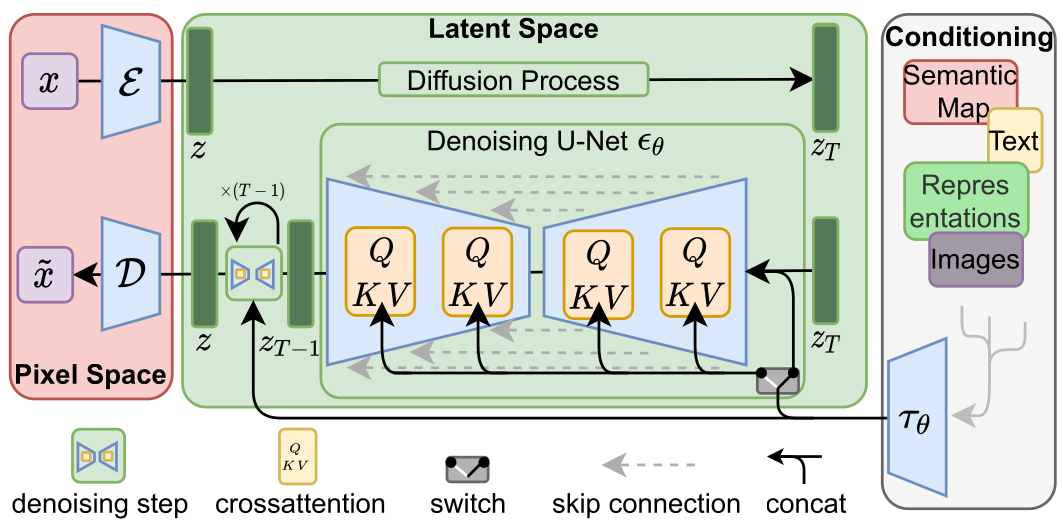
\includegraphics[width=0.95\linewidth]{ldm_arch.png}
	\caption{Architecture of Latent Diffusion Models, adapted from Rombach et al. \cite{Rombach_2022_CVPR}.}
	\label{fig:ldm_arch}
\end{figure}

%-------------------------------------------------------------------------
\subsection{Strengths and Limitations}

The combination of Latent Diffusion Models and CLIP represents a true milestone in the field of text-to-image generation, and while their architecture presents some considerable strengths, it still has to deal with critical limitations, particularly concerning structural control.

\textbf{Strengths.} First of all, the introduction of compressed latent space allows LDMs to drastically reduce computational costs and to accelerate the generative process, effectively making it more practical to work with high-resolution images.
Additionally, the abstract representation in latent spaces can be exploited to capture more general semantic features of the data, leading to more accurate and coherent outputs.
Another remarkable capability is that, due to the central role of CLIP embeddings, these models excel at zero-shot generation: they have the ability to interpret complex textual descriptions, blend different styles and represent novel concepts, even if they have never been trained on that specific example, without missing any of the features required in the prompt.

\textbf{Limitations.} The primary concern for the accuracy of LDMs and, in general, pure text-to-image models is that natural language is a one-dimensional sequence of tokens and is not always a strong control tool. Text prompts give semantic constraints, but not precise spatial structure for 2D or 3D geometrical coordinates, such as distance, orientation and exact positioning of the objects. Because of this lack of explicit geometric structure, the model is forced to ``guess'' the correct structural layout, only based on the training examples. As demonstrated by recent comprehensive benchmarks like \cite{NEURIPS2023_f8ad010c}, this spatial ambiguity issue can lead to physical inconsistencies, resulting in mistakes such as intersecting shapes, floating objects, incorrect proportions or wrong spatial positioning. In particular, for rigorous scientific fields requiring high accuracy, such as the one we are mainly interested in, forensic science, relying solely on textual prompts is insufficient for an exact description of the visual reconstruction needed. A sequence of language tokens cannot guarantee precise adherence to specific architectural structures, and exact depth maps or perspective constraints are required.

%-------------------------------------------------------------------------
\subsection{ControlNet Architecture}

To overcome the spatial limitations of pure text-to-image models, Zhang and Agrawala \cite{Zhang_2023_ICCV} introduced ControlNet, a neural network architecture specifically designed to add explicit spatial conditioning to large, pre-trained text-to-image diffusion models, such as LDMs.

\textbf{Architecture and Freezing Strategy.} A key characteristic of ControlNet is that it preserves the generative capacities of a pre-trained Latent Diffusion Model (such as Stable Diffusion) while adding new conditioning capabilities by introducing spatial constraints. To achieve this, instead of significantly modifying the original U-Net, its pre-trained weights are frozen, and a trainable copy of the encoding layers is created to form a new control branch. This implementation in the ControlNet architecture ensures that none of the massive semantic knowledge learned by the base model is lost, but also adds a new explicit and strong conditioning on the spatial structure.
This spatial conditioning is achieved through Control Maps, such as Depth Maps for the comprehension of 3D space and perspective, Canny Edges for precise outlines, Semantic Segmentation for precise object classification, Human Pose for an accurate depiction of human poses, and Normal Maps for the calculation of lighting and shadow positioning.

\textbf{Zero-Convolutions and Decoupling.} The communication between the frozen network and the trainable control branch is handled by a mechanism called \textit{Zero-Convolutions}. They consist of $1 \times 1$ convolutional layers where weights and biases are initialized to zero. Thanks to this initialization, during the first step, before the start of the actual training, the ControlNet branch outputs zero, leaving the original LDM completely unaffected and conserving its capabilities. As the training proceeds, the zero-convolutions gradually learn how to insert the geometric features from the Control Maps into the diffusion process. Finally, the resulting system decouples the generation process: the text prompt, which is processed via CLIP and the frozen LDM, controls the semantic content and style, while the spatial conditioning image, processed via ControlNet, dictates the rigid spatial structure of the output.
The introduction of this precise spatial control is what makes ControlNet such a powerful tool for all the applications requiring high geometrical accuracy, such as forensic science.

\begin{figure}[htbp]
	\centering
	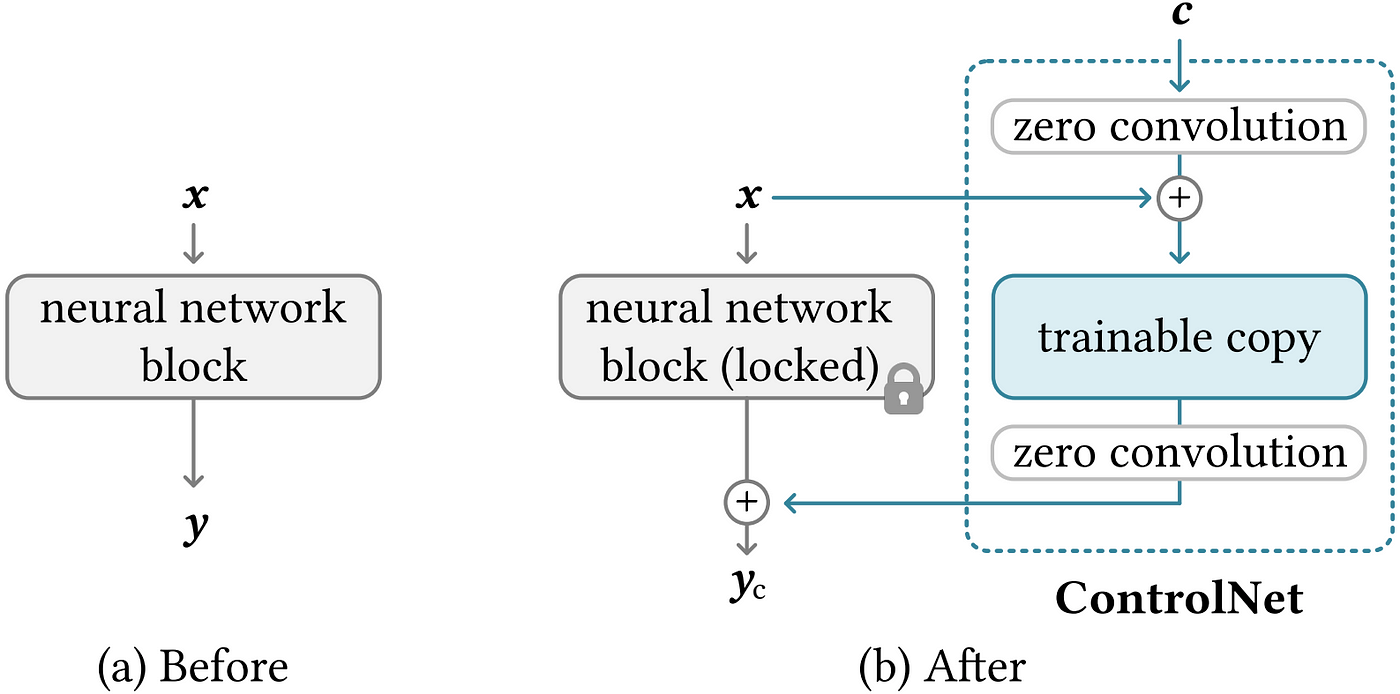
\includegraphics[width=0.85\linewidth]{controlnet_arch.png}
	\caption{The ControlNet architecture, adapted from Zhang et al. \cite{Zhang_2023_ICCV}.}
	\label{fig:controlnet_arch}
\end{figure}

%-------------------------------------------------------------------------
\section{Proposed Application: Forensic Scene Reconstruction}


The integration of ControlNet enables the combination of subjective elements, such as textual prompts, with objective constraints, such as precise spatial geometry. This capability is particularly relevant for the proposed application in forensic science. 

In a typical investigation, eyewitness testimonies provide a textual description of the crime scene from a subjective point of view, which is inherently prone to inaccuracies regarding the precise spatial positioning of elements. On the other hand, 3D Laser Scans utilized by forensic teams provide an objective geometric reconstruction, extremely accurate in mapping the exact spatial structure of the environment.

\subsection{Combining Laser Scans and Eyewitness Testimonies}

The aim of the proposed pipeline is to establish a connection between physical evidence and human memory by defining a multi-step process. In modern forensic investigations, the use of Terrestrial Laser Scanning (TLS) \cite{diagnostics13203169, forensicsci1020008} has become a common procedure to freeze the crime scene in its unaltered state and precisely reconstruct its dynamics, especially in complex cases, or in circumstances with a high risk of evidence contamination or degradation. High-precision devices, such as FARO or Leica laser scanners, are employed following strict institutional protocols \cite{ftcoe2022guidelines} to generate dense 3D point clouds. These scans calculate distances with remarkable precision due to the deployment of lasers and map the exact geometry of the environment, including the size and positioning of furniture, walls and objects.

The 3D environment produced is objectively accurate, but needs to be converted to a 2D space to enable the application of Latent Diffusion Models. The method requires an intermediate extraction step: using the 3D point cloud data, investigators can position a virtual camera exactly at the location and height where the eyewitness claimed to be standing. From this viewpoint, the 3D software can render a precise 2D Depth Map, consisting of a grayscale image representing the exact distance of every surface from the witness's perspective. Following this procedure, the scanned 3D geometry can be projected into a 2D representation without losing depth information.

After the generation of spatial constraints, the ControlNet architecture can be deployed. The trainable control branch can utilize the rendered depth map, as previously described, to impose a rigid spatial conditioning on the architecture of the scene. Simultaneously, the textual prompt derived from the eyewitness testimony (e.g., ``a male suspect wearing a blue coat standing next to the door'') is processed via CLIP to guide the Latent Diffusion Model. The union of the semantic elements (people, clothes, actions, lighting) and the geometric boundaries imposed by the laser scan produces a realistic 2D representation of the eyewitness point of view.

\subsection{Utility in Forensic Investigations}

The application of this generative method introduces significant advantages across multiple phases of the investigation and judicial process. Primarily, it could act as a powerful tool during the early phases of an investigation: by generating multiple visual scenarios based on different textual hypotheses, detectives can explore alternative crime dynamics and formulate new investigative hypotheses. 

Another important advantage is the ability to assess the reliability of eyewitness accounts: by pairing a subjective testimony with the objective constraints of the 3D scan, investigators can verify the physical plausibility of a statement. For instance, evaluating line-of-sight constraints would be much easier with the help of a visual support, confirming whether a witness could have actually seen a specific detail from their declared position. Additionally, multiple witnesses could provide conflicting testimonies, and generating images of each testimony within the same spatial environment can highlight inconsistencies and guide further interrogations.

Beyond the investigative phase, this approach offers substantial benefits also during legal proceedings. Interpreting black-and-white 2D floor plans or 3D point clouds can be challenging for an ordinary jury, not composed of experts in the field. The proposed method acts as an effective tool for a practical visualization of abstract data and spoken testimonies and could be integrated as a support in court evaluation. However, it is crucial to point out that these generated images cannot be presented as forensic evidence, but rather as simple tools designed to help the jury visualize the scene and evaluate the plausibility of the narratives presented in court.

A possible direction for future work in the field would be to evaluate the consistency between generated images and ground-truth geometry, as well as the agreement across multiple independent testimonies.

\subsection{Critical Issues and Ethical Limitations}

Despite the possible advantages previously described, the proposed application presents significant critical issues and ethical concerns. First of all, even sophisticated models such as LDMs and ControlNet are not perfect and can suffer from ``hallucinations'': neural networks cannot truly understand real-world logic, which can lead to critical mistakes, such as the generation of objects in different positions than those described by the eyewitness, or the alteration of fundamental characteristics in the suspect's physical appearance. One of the possible mitigations for this issue could be uncertainty modeling: generating a distribution of images instead of a single output, or including the eyewitness in the generation process through an iterative selection of the most accurate representations.

Another major criticality is confirmation bias. When a jury is shown a highly plausible visual representation, they are naturally inclined to believe in its truthfulness. The human brain is inherently predisposed to trust what it sees, raising the risk that photorealistic generated images could be wrongly interpreted as absolute truth or real-life photographic evidence, overshadowing the possibility of mistakes in the testimonies due to lack of memory or deceiving intentions.

\section{Conclusion}

In conclusion, this essay has explored the architecture of Latent Diffusion Models (LDMs) and their significant capabilities in text-to-image generation. While these models present extraordinary zero-shot generation skills, they suffer from critical limitations regarding spatial ambiguity and geometric accuracy. As discussed, the introduction of explicit spatial conditioning through ControlNet helps mitigate the issue.

Building upon these technical foundations, we proposed an application for forensic scene reconstruction. By merging the subjective, semantic descriptions of eyewitness testimonies with the objective, precise geometric data provided by 3D Terrestrial Laser Scans, this method offers a new visualization tool for investigators and legal proceedings. Although the approach presents critical challenges such as AI hallucinations and confirmation bias, the controlled integration of generative AI into forensic science constitutes a promising tool for applications in modern investigations.


{\small
\bibliographystyle{ieee_fullname}
\bibliography{ATDS_essay_RiccardoPilan}
}

\end{document}
